%!TEX root = ../report.tex
\documentclass[../report.tex]{subfiles}
\begin{document}
    \chapter{Background}\label{chap_background}
	Last chapter introduced the reader to this research work by discussing its objectives and formulating them into research questions. This chapter provides the necessary background information for the reader to understand this research work. It begins with a description of GestaltMatcher's working and how it surpasses human performance in diagnosis of rare genetic syndromes from facial images. Subsequently, an introduction to the topic of Explainable Artificial Intelligence (XAI) is given. Information on the genetic syndromes considered for this research work is provided alongside their respective result discussions in Chapter 6 for ease of reading. 
    \section{Genetic Syndrome Diagnosis using GestaltMatcher}
    GestaltMatcher is a state-of-the-art (SOTA) neural network based tool developed to diagnose rare genetic syndromes from frontal facial images of people. It surpasses the ability of clinicians to recognize images of certain rare genetic conditions. GestaltMatcher stands out from the rest of all similar works for its ability to diagnose a patient even if the disorder he/she suffers was not a part of the training set.\\ 
    In the beginning, we describe the construction of GestaltMatcher. Subsequently, we explain the two applications of the tool. Finally, we provide details about GestaltMatcher's performance on the GestaltMatcherDataBase (GMDB) dataset.     
    \subsection{Construction}
    Under the hood GestaltMatcher consists of a  Convolutional Neural Network (CNN) based encoder which acts as a feature extractor
    to transform inputted images into embeddings in a highly discriminative embedding space. Patient photos from datasets such as GMDB are pre-processed before feeding them into the encoder.
    The pipeline shown in Figure \ref{fig_gm_pipeline_ch2} illustrates the sequence of steps involved in processing a patient photo using GestaltMatcher.
    \begin{figure}[ht]
    	\hspace*{-0.5cm}      
    	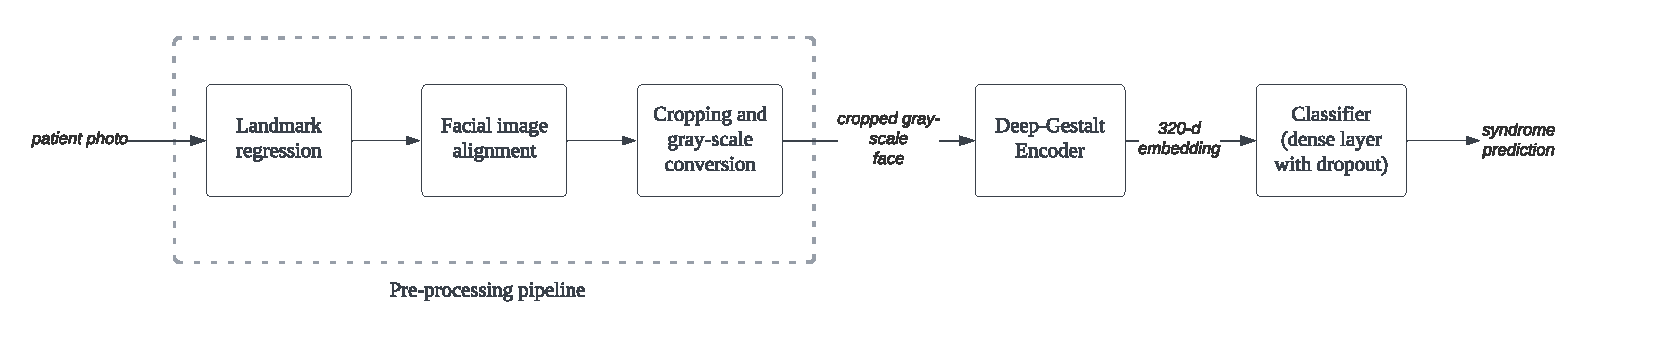
\includegraphics[scale=0.65]{chapter2/gestalt_matcher_pipeline.pdf}
    	\caption{Illustration of the pipleline to process a patient photo using GestaltMatcher}
    	\label{fig_gm_pipeline_ch2}
    \end{figure}
    
    \subsubsection{Pre-processing Pipeline}
    The pre-processing pipeline is responsible for detecting facial landmarks and aligning the orientation of a given patient photo, and finally cropping the face from it. Authors of GestaltMatcher use RetinaFace \cite{deng2020retinaface} to fetch detect landmark points from a patient's facial image.  In a nutshell, RetinaFace is a single-stage, multi-scale face localization method which employs multi-task learning to perform five different tasks: face detection, landmark position and score regression,  3D position and pixel correspondence prediction. It uses a Resnet-50 \cite{he2016deep} backbone. The facial landmark coordinates outputted by RetinaFace is used to crop and align faces from patient photos. The facial images are resized to 100 x 100, and converted to gray-scale before feeding them into the encoder module.
    
    \subsubsection{Deep Gestalt Encoder}
    The encoder in GestaltMatcher is called as \enquote{Deep Gestalt} encoder, named after the work \cite{Gurovich2019} in which its architecture was first proposed. The CNN based encoder consists of ten convolutional layers and uses Rectified Linear Unit (ReLU) activation function. Please refer Figure \ref{fig_arch_gest_matcher} in Chapter \ref{ch_implementation} an enumeration of the network architecture. Deep Gestalt encoder extracts features from input facial images and represents them in 320-dimensional embedding space called the Clinical Face Phenotype Space (CFPS). The embeddings in CFPS are called as Facial Phenotype Descriptors (FPDs). Authors of GestaltMatcher use the encoder differently for two of its applications: syndrome classification and patient matching.
    
    \subsection{Applications}
    An intuitive application of GestaltMatcher is genetic syndrome recognition. In this case, a dense layer which acts as a classifier is appended to the encoder. Top-k predictions within the scope of trained classes can be obtained for any patient's facial image. The GestaltMatcher classifier is useful when a clinical practitioner suspects his patient to have a particular genetic condition and seeks to validate his diagnosis.
    
    
    The primary application of GestaltMatcher is patient matching. CFPS acts as a discriminative embedding space to measure similarities between FPDs of patients with known or unknown disorders. The cosine similarity metric is used to quantify similarities between cases. The measure can computed using the following formula: 
 
    \begin{equation}
    	\cos ({\bf p},{\bf q})= {{\bf p} {\bf q} \over \|{\bf p}\| \|{\bf q}\|} = \frac{ \sum_{i=1}^{n}{{\bf p}_i{\bf q}_i} }{ \sqrt{\sum_{i=1}^{n}{({\bf p}_i)^2}} \sqrt{\sum_{i=1}^{n}{({\bf q}_i)^2}} }
    \end{equation}
	where $p$ and $q$ represent vectors each of dimensions $n$.
    GestaltMatcher helps to perform an objective comparison of patients with same or different disorders, with shared phenotypic features. Authors of GestaltMatcher provide an example for such an application scenario, and describe how the tool was used to match patients from different families, who suffered from the same disorder. 
    
    Besides diagnosing known disorders, GestaltMatcher can be used to identify novel genetic conditions. For example, when a syndromologist is unable to find the molecular cause for a patient's phenotype, he/she could use the matching tool, to match the case's FPD with the existing instances in the CFPS. Position of the FPD can be used to determine whether the patient suffers from an unidentified disorder. The CFPS neighborhood of such a case can be used in the identification of genes associated with the unknown disorder. 
    \begin{figure}[ht]
    	\hspace*{1.0cm}      
    	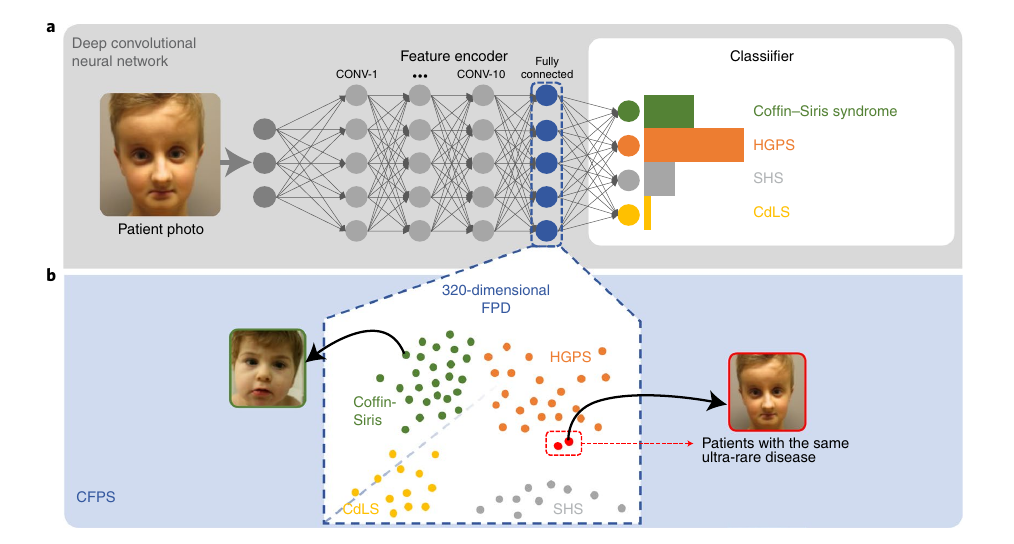
\includegraphics[scale=0.4]{chapter2/gestalt_matcher_application.png}
    	\caption{Use cases of GestaltMatcher: a. syndrome classification b. patient matching. Image source: \cite{hsieh2022gestaltmatcher} (p.3) }
    	\label{fig_app_gest_matcher_chap2}
    \end{figure}
    \subsection{Performance}
    GestaltMatcher achieves state-of-the-art performance in the task of syndrome recognition, measured using the top-k accuracy metric. Its authors report the model's performance on two datasets: Face2Gene, a propreitary one, and GMDB, which consists of images obtained from 902 scientific publications. The model's performance on GMDB is presented in the table below, as the same dataset was used for our research work.  
    \section{Introduction to XAI}
	\enquote{XAI is artificial intelligence (AI) in which humans can understand the decisions or predictions made by the AI}\cite{vilone2021notions}. It also refers to a branch of study which deals with the development of processes and methods to explain decisions of AI systems. The \enquote{interpretability} is often used interchangeably with \enquote{explainability}. However, it is important to note that interpretability has to do with describing the internals of an AI system, in a way that is understandable to humans. In this section, we give an overview of different types of methods developed to visualize internals of neural network models, especially CNNs such as the one used in GestaltMatcher, and explain their predictions.
	
	\subsubsection{Methods for Neural Networks}
	Figure \ref{} depicts the taxonomy of explanation methods for neural network methods as presented in \cite{molnar2019}. 
	
	\subsubsection{Feature Visualization}
	This class of methods focus on visualizing features learned in hidden layers of a CNN. Entities like edges, textures, patterns, parts and objects can be visualized by maximizing activations of convolutional layers. Last layers of neural network model learn features of higher complexity than the earlier ones.  Feature visualization can be achieved through optimization, or by using approaches such as network dissection \cite{bau2017network}, in which highly activated channels of a given layer are associated with human concepts such as color. Although feature visualization seems to be a simple tool for understanding internals of a neural network, often its visualization artifacts are not interpretable. Besides, another challenge lies in choosing the right set of layers and channels for visualization, and summarizing information represented in them.

	\subsubsection{Attribution Methods}
	Attribution methods provide the rationale behind a CNN model's output by producing an attribution map representation, in which every pixel or feature of the input image is assigned a score based on how much it impacts a given prediction. Artifacts generated by attribution methods are called with different names like saliency maps, attribution maps and sensitivity maps, based on the approach used to generate them.
	
	Attribution methods can be categorized in two types, based on how they compute attribution scores:  perturbation/occlusion-based and gradient-based. Perturbation methods manipulate sections of the input to compute their importance scores. On the other hand, gradient-based methods make use of gradient information obtained by computing derivatives of output score with respect to feature values to calculate attributions. This research work uses attribution methods to understand GestaltMatcher's regions of attention in syndromic faces and to explain its predictions.
	\subsubsection{Concept Visualizations}
	Concept based approaches are built with an intent to detect and visualize user-defined concepts such as a patterns or any abstraction in the latent space learned by a neural network model.  Testing with Concept Activation Vectors (TCAV) \cite{tcav} can be taken as an example for a concept visualization method. It quantifies any given concept's influence on a neural network model's prediction for a given class.
	
	\subsubsection{Influential Instances}
	A training data sample is considered \enquote{influential} when its deletion from the train set considerably affects the predictions of a model. Identification of influential instances offers a way to debug machine learning models and explain their predictions.
	
	\subsubsection{Counterfactual Explanations}
	A counterfactual explanation of a model prediction explains the least change to the input feature values which changes the prediction to a predefined output. Adversarial examples \cite{} make a great example for counterfactual explanations. However, they are synthesized with an intent to deceive a model rather than explaining its predictions.
\end{document}